\documentclass{article}
\usepackage{enumitem,graphicx,xcolor, booktabs}
\usepackage[colorlinks=true, urlcolor=black, linkcolor=black,citecolor=black]{hyperref}
\usepackage[margin=1in]{geometry}
\usepackage[]{units}
\begin{document}
 \graphicspath{{imgs/}} 
 
 
 {\color{red}
   \begin{itemize}
   	\item Numerical labels are hard to read for Figure \ref{fig:overall-f} both main panel and inset. Rewrite them with LaTeX?
   	\item Add table to define abbreviations such as LSD, DMT, \ldots
   	\item Axes for Figure \ref{fig:pca} should all range from $-1$ to $1$. 
   	\item Include scree plot and silhouette score plot for Figure \ref{fig:pca}
   	\item Make Table of Bonferonni corrected p-values for significant correlations in Figure \ref{fig''drug-drug-correlation}
   \end{itemize}
 }
 
\section*{Methods}

 \emph{Acquisition of data}
 	We used Scrapy \cite{myers2015} to scrape text from all fora in \href{http://www.lycaeum.org}{Lycaeum} in December $2015$. The analyses in this paper reflect the content of Lycaeum at that time. 
 
\emph{Preprocessing of data}	
 	
\emph{Analysis of data} To quantify how similar the drugs were in two documents we used the Jaccard similarity (citation). The Jaccard similarity between two objects is the ratio of the components those objects share in common to the number of unique elements in either object. It is the ratio of intersection of the sets of components of two objects to the union. We chose Jaccard similarity over cosine distance because cosine distance considers two objects with binary features similar if they both lack the same feature. It did not seem reasonable to consider to posts related if they both failed to mention one of $802$ drugs. 
 
\section*{Results}

\emph{Patterns of drug use}
  Figure \ref{fig:overall-f} shows the twenty most frequent substances mentioned in the Lycaeum corpus. The main panel of Figure \ref{fig:overall-f} shows the top \nicefrac[]{20}{161} most mentioned substances across the Lycaeum corpus. We include ``sound'',  a common ``coingestant'' with LSD, when we write \emph{substance}.  It is not surprising that LSD is mentioned more often than caffeine or ethanol. Lycaeum aims to provide information about psychoactive substances. 
  
  Figure \ref{fig:drug-drug-correlation} shows the pattern of co-mentions of pairs of substances. In Figure \ref{fig:drug-drug-correlation} the color of the $ij$th square represents the Spearman correlation between number of documents mentioning drugs $i$ and $j$ in the corpus. To determine which correlations were significant we calculated the adjusted two-tailed p-value for each correlation coefficient for each combination of drugs. We adjusted each p-value by applying the Bonferroni correlation, assuming that we were testing for $47$ hypotheses (drug-drug pairs) simultaneously. Table X lists the combinations that occurred statistically significantly more frequently than would be expected by chance. 
  
  \begin{figure}[h]
\centering
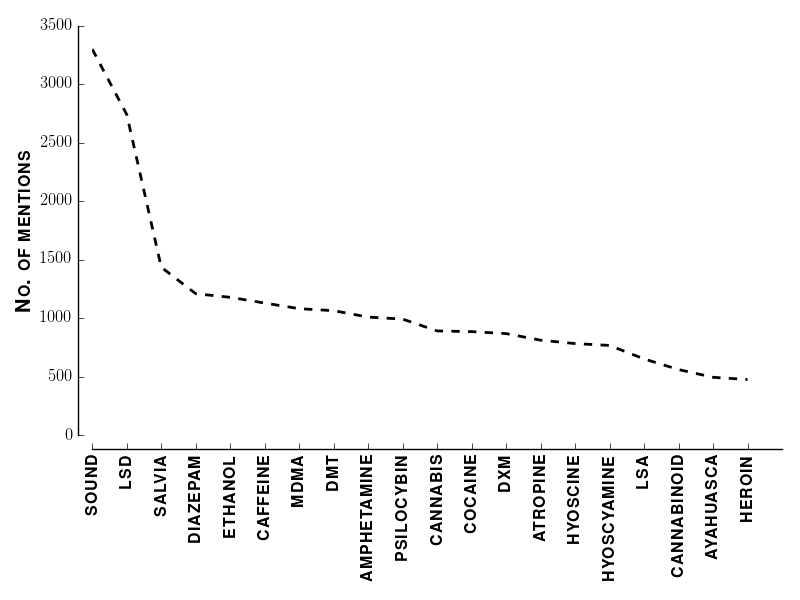
\includegraphics[scale=0.65]{overall-drug-frequency.png}
\caption{\textbf{Overall frequency of substance mentions.} $20$ most prevalent substances are shown. Refer to Table X for abbreviations. \textbf{Inset:} Distribution of number of mentions of drugs across corpus. Main figure is derived from portion of histogram to the right of the vertical red line.}
\label{fig:overall-f}
\end{figure}
  
\emph{Patterns of effects}
  Figure \ref{fig:effect-f} shows the twenty most frequent effects mentioned in the Lycaeum corpus. Table \ref{tab:effect-defs} presents the definitions of some effects in Figure \ref{fig:effect-f} that may be unfamiliar to the reader. Nearly all drugs mentioned in the Lycaeum corpus have multiple effects. For some, such as the opioids, anticholinergics, and stimulants, the dose determines which effect predominates. We did not attempt to infer dose from Lycaeum. There is no way to verify reported doses. One way to better understand dosage is to compare the doses mentioned across multiple websites similar to Lycaeum. 

\begin{table}[h]
\centering
\begin{tabular}{@{}ll@{}}
\toprule
Term         & Connotation                                                                    \\ \midrule
Entactogen   & Feelings of belonging, familiarity, emotional openness; also called empathogen \\
Entheogen    & Altered consciousness with religious, spiritual overtones                      \\
Hallucinogen & Perception of something without any sensory input                              \\
Psychedelic  & Alters perception and cognition                                                \\ \bottomrule
\end{tabular}
\caption{Terms used in x-axis of Figure \ref{fig:effect-f}}
\label{tab:effect-defs}
\end{table}

   We hypothesized that users mix psychoactive substances to achieve distinct combinations of effects. We assumed that discussions on Lycaeum, at least in the aggregate, faithfully report that mixing. To test this hypothesis we investigated whether some pairs or groups of effects were mentioned together more frequently than others.
   
     To identify  we calculated the frequency with which pairs of effects were mentioned 
   
   


\begin{figure}[h]
\centering
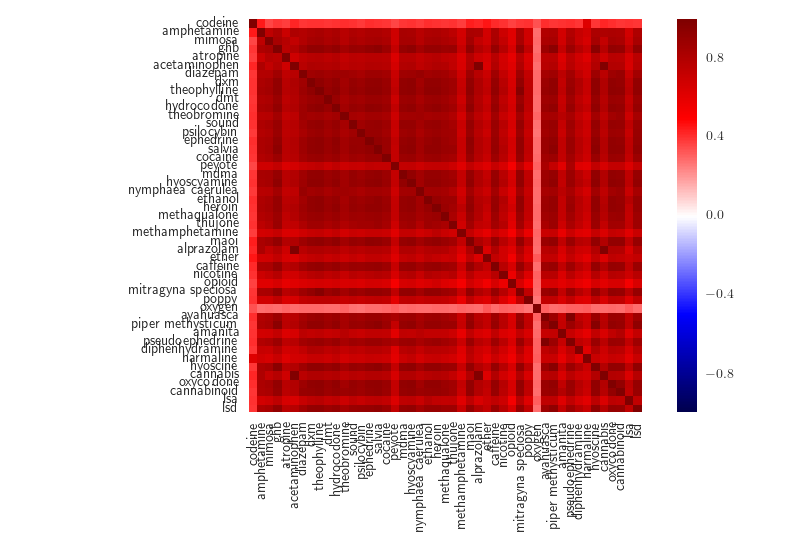
\includegraphics[scale=0.65]{drug-correlation-matrix.png}
\caption{\textbf{Co-mentions of drugs.} Each square of the heat map shows the Spearman correlation between the substances indicates in the intersecting row and column. Warmer colors designate stronger positive correlation. Cooler, stronger negative correlation. }
\label{fig:drug-drug-correlation}
\end{figure}

\begin{figure}[h]
\centering
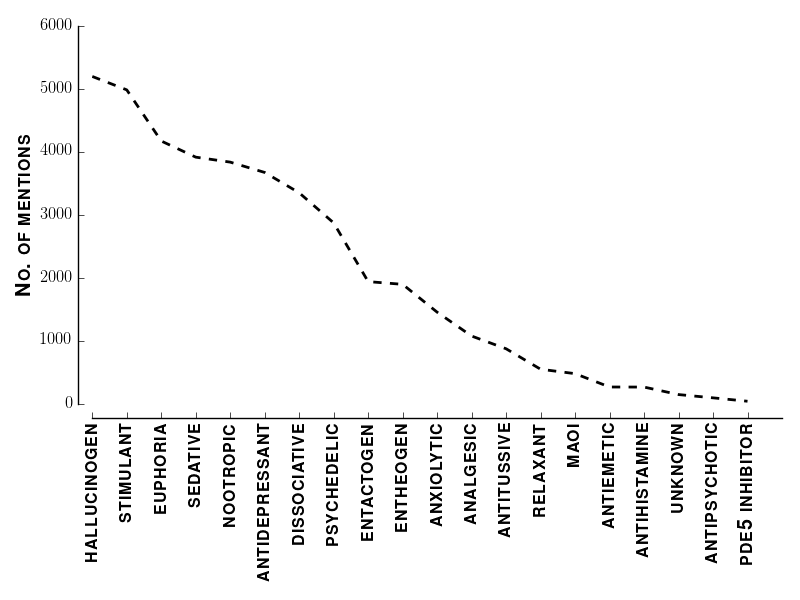
\includegraphics[scale=0.65]{effect-frequency.png}
\caption{\textbf{Overall frequency of substance effects.}}
\label{fig:effect-f}
\end{figure}

\begin{figure}[h]
\centering
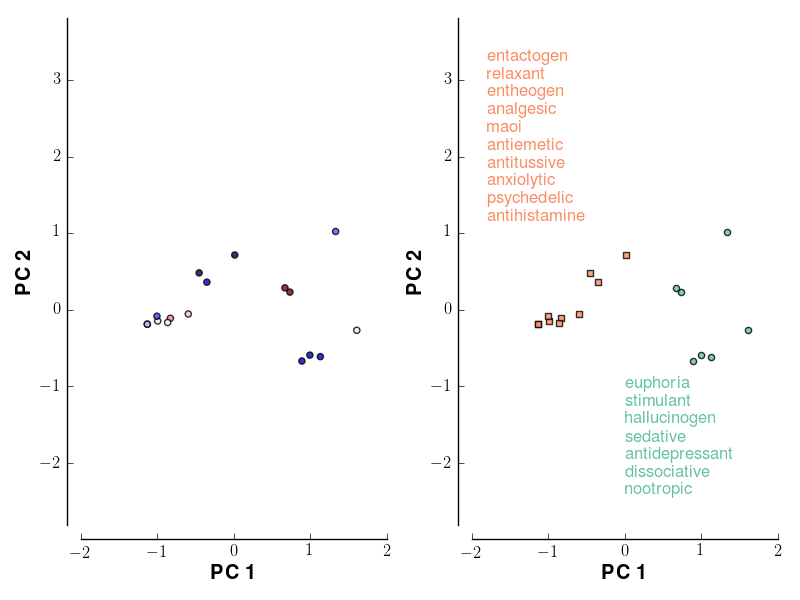
\includegraphics[scale=0.65]{effect-matrix-pca-w-clusters-g.png}
\caption{\textbf{Scatter plot of drug class combinations. Left: }Projection of drug effect combinations on first two principal components. \textbf{Right:}}
\label{fig:pca}
\end{figure}

\bibliographystyle{unsrt}
\bibliography{bibliography}

\end{document}